\documentclass[a4paper,12pt,openany]{book}
\usepackage [utf8]{inputenc}
\usepackage [french]{babel}
\usepackage [T1]{fontenc}
\usepackage{listings}
\usepackage{graphicx}
\usepackage{verbatim}

%%configuration de listings
\lstset{
language=c,
basicstyle=\ttfamily\small, 
identifierstyle=\color{red}, 
keywordstyle=\color{blue}, 
stringstyle=\color{black!60}, 
commentstyle=\it\color{green!95!yellow!1}, 
columns=flexible, 
tabsize=1, 
extendedchars=true, 
showspaces=false, 
showstringspaces=false, 
numbers=left, 
numberstyle=\tiny, 
breaklines=true, 
breakautoindent=true, 
captionpos=b
}

%coloration syntaxique
\usepackage{xcolor}
\definecolor{Zgris}{rgb}{0.87,0.85,0.85}

\newsavebox{\BBbox}
\newenvironment{DDbox}[1]{
\begin{lrbox}{\BBbox}\begin{minipage}{\linewidth}}
{\end{minipage}\end{lrbox}\noindent\colorbox{Zgris}{\\usebox{\BBbox}}
[.5cm]}

%Pour l espace entre la section et la chapitre (qui est trop grand).
\usepackage{titlesec}

\titleformat{\chapter}[block]
  {\normalfont\Huge\bfseries}% font of number
  {\chaptertitlename\ \thechapter~:}% format of number
  {20pt}% space between number and title
  {\Huge}% font of title

\titlespacing*{\chapter}
  {0pt}%  indent
  {0pt}% space before
  {20pt}% space after
\titlespacing*{\section}
  {0pt}%  indent
  {3.5ex plus 1ex minus .2ex}% space before
  {2.3ex plus .2ex}% space after

\author{Mendy Fatnassi}
\title{Programmation Orienté Objet}




%%%%%%%%%%%%%%%%%%%%%%%%%%%%%%%%%%%%%%	Page	%%%%%%%%%%%%%%%%%%%%%%%%%%%%%%%%%%%%%%%%

\begin{document}
\maketitle
\tableofcontents

\chapter{POO}


\section{Langage Orienté Objet}

\begin{flushleft}
Un Langage Orienté Objet (LOO) $\neq$ Langage Objet (LO).\\
Il existe plusieur langage utilisant les principe de la POO tel que : Ruby,JAVA,C++,SmallTalk,Eiffel,Ada,Python,...\\
\end{flushleft}

%%%%%%%%%%%%%%%%%%%%%%%%%%%%%%%%%%%%%%%%%%%%%%%%%%%%%%%%%%%%%%%%%%%%%%%%%%%%

\section{Notion et Concept de base}

\subsection{Objet}: \\

\textbf{Identité}: Signifie que les données sont regroupés en entités discrètes et identifiables appelés objets.\\

\begin{flushleft}
Dans le monde réel nous somme entouré d'objet tel que une chaise, une voiture, une table ,etc. Ces objets posséde:\\
-Des propriété, la chaise possède 4 pieds, elle est de couleur bleue, etc.\\
-Peuvent faire des actions, la voiture peut rouler, klaxonner, etc.\\
-Ils peuvent également interagir entre eux (l’objet conducteur démarre la voiture, l’objet voiture fait tourner l’objet volant, etc.).\\
Sachant qu’un objet en programmation c’est comme un objet du monde réel mais ce n’est pas forcément restreint au matériel. Un chien est un objet. Des concepts comme l’amour ou une idée sont également des objets, tandis qu’on ne dirait pas cela dans le monde réel.\\
\\
Un objet est responsable des valeurs des variables d'etat (attributs).\\
\end{flushleft}

%%%%%%%%%%%%%%%%%%%%%%%%%%%%%%%%%%%%%%
\subsection{Instance}: \\

\begin{flushleft}
Il faut bien faire attention à distinguer ce qu’est l’objet et ce qu'est la définition d’un objet.\\
La définition de l’objet (ou structure de l’objet) permet d’indiquer ce qui compose un objet, c'est-à-dire quelles sont ses propriétés, ses actions etc. Comme par exemple le fait qu’une chaise ait des pieds ou qu’on puisse s’asseoir dessus.\\
Par contre, l’objet chaise est bien concret. On peut donc avoir plusieurs objets chaises : on parle également d’\textbf{instances}.\\
\end{flushleft}

%%%%%%%%%%%%%%%%%%%%%%%%%%%%%%%%%%%%%%
\subsection{Class}: \\

Un objet (concret) peut etre definit par une classe (objet abstrait).\\
Une instance d'une class est un objet.\\\\
Par exemple si on prend ce texte :\\
"un compte en banque \emph{connait} un numero, un titulaire et un solde et \emph{est capable} de donner le solde, de deposer une somme et de retirer une somme "\\
\\
-Ce texte definit monCompte,tonCompte,sonCompte,unAutreCompte etc..\\
-Et definit la class Compte a partir de laquelle on pourras creer tous les autres comptes particulier.\\
\\
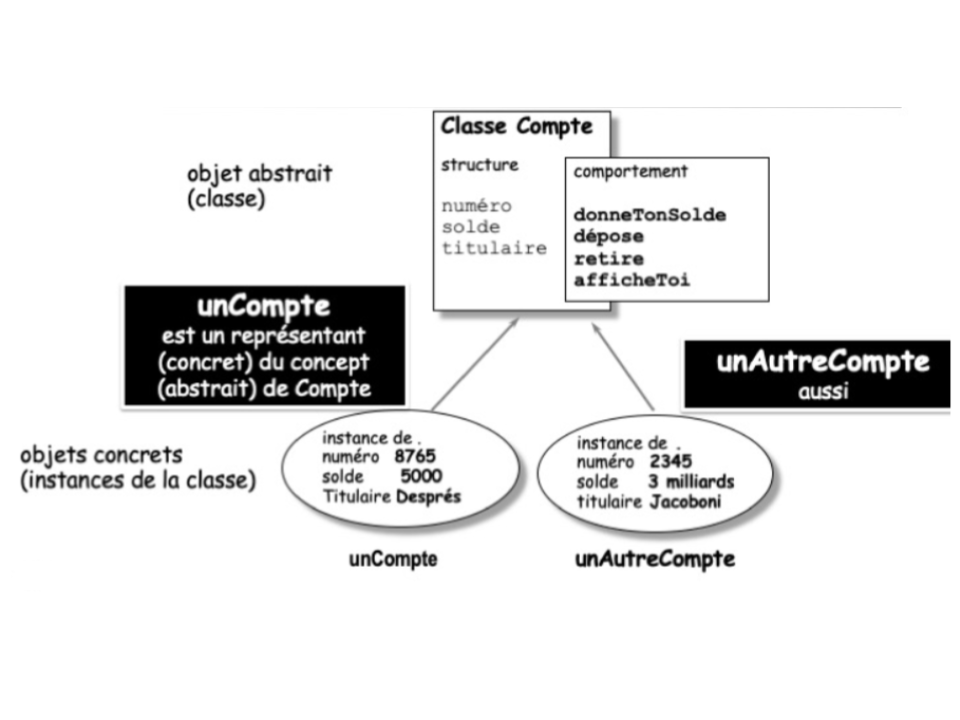
\includegraphics[width=1,\linewidth,center]{img/exemple-class.png}
\\
Une classe est donc structuré de la facons suivante:\\
-Une liste de noms de champs (variables d'instances).\\
-Un catalogue de procédures (méthodes).\\
\\
\textbf{Methode de class}:\\
A ne pas confondre avec une methode d'instance qui agit que sur un seul objet (instance de classe) a la fois.\\
Une methode de class (statique) est indépendante de toute instance de la classe.\\

%%%%%%%%%%%%%%%%%%%%%%%%%%%%%%%%%%%%%%
\subsection{Methode}: \\
Il s'agit du comportement d'un objet decrit par un ensemble de procédure (opération).\\
Appelé fonction membres (en C++), méthode (en ruby.\\


%%%%%%%%%%%%%%%%%%%%%%%%%%%%%%%%%%%%%%
\subsection{Interface}

On ne peut communiquer avec un objet que par son interfaces (les services qu'il offrent).\\


%%%%%%%%%%%%%%%%%%%%%%%%%%%%%%%%%%%%%%%%%%%%%%%%%%%%%%%%%%%%%%%%%%%%%%%%%%%%

\section{Concepte fondamentaux de la POO}:\\
\\

\textbf{Variable d'etat d'un objet}: Il s'agit de champs qui serve a decrire la class.\\ 
Appelé données membres (en C++), \textbf{Variable d'instance} (en Ruby).
\\
\textbf{Message}: Un objet (emetteur) envoie un message a un objet (receveur). Un message permet d'activer une méthode de l'objet receveur.\\
En reponse a un message l'objet destinataire du message déclenche un comportement.\\ 

%%%%%%%%%%%%%%%%%%%%%%%%%%%%%%%%%%%%%%
\subsection{Heritage}: \\

C’est-à-dire qu’un objet dit "père" peut transmettre certaines de ses caractéristiques à un autre objet dit "fils".\\
Pour cela, on pourra définir une relation d’héritage entre eux. S’il y a une relation d’héritage entre un objet père et un objet fils, alors l’objet fils hérite de l’objet père. On dit également que l’objet fils est une \textbf{spécialisation} de l’objet père ou qu’il dérive de l’objet père.\\
A l'inverse on peux adopter une méthode de \textbf{généralisation} de l'objet père càd on commence par definir l'objet fils et ensuite on definit l'objet père (le fils heritera tout pareil du père).\\ 
\\
Grace a cela nous pouvons etablir une hiéarchie des classes. exemple:\\
\\
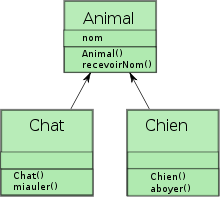
\includegraphics[width=0.35\linewidth,center]{img/poo-heritage.png}

%%%%%%%%%%%%%%%%%%%%%%%%%%%%%%%%%%%%%%
\subsection{Classification}: \\

Les objets ayant la meme structure de données et les memes services sont regroupés dans une classe.\\

%%%%%%%%%%%%%%%%%%%%%%%%%%%%%%%%%%%%%%
\subsection{Abstraction}: \\

L'abstraction est une vue générique d'une entité permettant de ne pas etre limité par des contraintes technique ou matériel.\\
Par exemple la structure personne peut definir une infinité d'objet qui seront isomorphe (meme structure), on auras donc plusieurs personne (pers1,pers2,...).\\
Leurs comportement seras identique car ils partagent l'ensemble des procédures.\\
Le texte definissant un objet (concret) devient une classe (objet abstrait) définissnt une infinité d'instances.\\


%%%%%%%%%%%%%%%%%%%%%%%%%%%%%%%%%%%%%%
\subsection{Polymorphisme}: \\

Le mot polymorphisme suggère qu’une chose peut prendre plusieurs formes. Sous ce terme un peu barbare se cachent plusieurs notions de l’orienté objet qui sont souvent sources d’erreurs.\\
\\
C'est la capacité pour un objet de faire une même action avec différents types d’intervenants. C’est ce qu’on appelle le polymorphisme "ad hoc" ou le polymorphisme "paramétré".\\
\\
Par exemple, notre objet voiture peut rouler sur la route, rouler sur l’autoroute, rouler sur la terre si elle est équipée de pneus adéquats, rouler au fond de l’eau si elle est amphibie, etc.\\
Concrètement ici, je fais interagir un objet "voiture" avec un objet "autoroute" ou un objet "terre", par l’action qui consiste à "rouler".\\

\textbf{La substitution} est une autre manifestation du polymorphisme. Il s’agit de la capacité d’un objet fils à redéfinir des caractéristiques ou des actions d’un objet père.\\
\\
Prenons par exemple un objet mammifère qui sait faire l’action "se déplacer". Les objets qui dérivent du mammifère peuvent potentiellement avoir à se déplacer d’une manière différente. Par exemple, l’objet homme va se déplacer sur ses deux jambes et donc différemment de l’objet dauphin qui se déplacera grâce à ses nageoires, etc.\\
\\
Tous ces mammifères sont capables de se déplacer, mais chacun va le faire d’une manière différente. Ceci est donc possible grâce à la substitution qui permet de redéfinir un comportement hérité. Ainsi, chaque fils sera libre de réécrire son propre comportement, si celui de son père ne lui convient pas.\\

%%%%%%%%%%%%%%%%%%%%%%%%%%%%%%%%%%%%%%
\subsection{Encapsulation}

En POO un objet a des donnée internes. Ces données sont spécifié dans la classe.\\
En ruby l'unité d'encapsulation est la classe.\\
Un objet est responsable de son fonctionnement, de ces méthodes, il ne se laisse pas manipuler par un autre objet.\\
Les objet vont plutot s'envoyer et manipuler des messages.\\
\\
L'écriture de classes offre d'autres avantages que le simple regroupement de données et de traitements. Parmi ceux-ci figure la possibilité de restreindre l'accès à certains éléments de la classe. C'est ce que l'on appelle l'encapsulation.\\
Exemple:\\
\\
\begin{verbatim}
class CompteBancaire
{
    private titulaire;   // attribut privé
    public solde;
    private devise;      // attribut privé
    ...
    du code
    ...
}
\end{verbatim}

À présent, la seule manière de définir des valeurs pour titulaire et devise est d'utiliser le constructeur. Toute tentative d'accès externe aux propriétés privées générera une erreur lors de la compilation.\\
\\
\begin{verbatim}
comptePierre = new("Pierre", 0, "euros");

comptePierre.titulaire = "Pierre";  // Erreur : titulaire est un attribut privé
comptePierre.solde = 500;           // OK : solde est un attribut public
comptePierre.devise = "euros";      // Erreur : devise est un attribut privé
\end{verbatim}
\\
Niveau d'encapsulation:\\
\\
- \textbf{public}: Les méthodes de la classe peuvent etre appelé depuis n'importe ou dans le code (classe par défaut public).\\
- \textbf{private}: La méthode ne pourra être appelée qu’à l’intérieur du code de la classe, sans indiquer de récepteur.\\
- protected : la méthode ne pourra être appelée qu’à l’intérieur du code de la classe ou de une de ses classes filles.\\
\\
\\
Encapsulation des attributs:\\
\\
En Ruby, tout attribut d’instance est par définition privé. Pour déclarer que l’on peut y accéder en lecture il faut définir une méthode d’accès en lecture grâce à la syntaxe : attr\_reader,attr\_writer ou  attr\_accessor . \\

%%%%%%%%%%%%%%%%%%%%%%%%%%%%%%%%%%%%%%%%%%%%%%%%%%%%%%%%%%%%%%%%%%%%%%%%%%%%

\section{Constructeur/Accesseur}

\underline{Constructeur} : methode initialize et new.\\
chaque appele de la methode new ferass automatiquement appele a initialize . Si initialize(param) a des parametre , alors la méthode new doit aussi avoir des paramétres.\\
\\
Un accesseur est une méthode le plus souvent publique qui permet d'accéder à un attribut privé.\\
\\
Un accesseur en lecture (getter) permet de lire la valeur d'un attribut.\\
Un accesseur en écriture (mutateur ou setter) permet de modifier la valeur d'un attribut.\\
\\
\verb+attr_reader :symbol[,:symbol]+ \\
\verb+attr_writer :symbol[,:symbol]+  \\
\\
On peux definir un raccourcie qui reunie les attribut en lecture et ecriture : attr\_accessor \\



%%%%%%%%%%%%%%%%%%%%%%%%%%%%%%%%%%%%%%%%%%%%%%%%%%%%%%% Ruby %%%%%%%%%%%%%%%%%%%%%%%%%%%%%%%%%%%%%%%%%%%%%%%%%%%%%%%%%%%

\chapter{Ruby}

\section{Généralité}

Ruby est un lagage open-source dynamique $\neq$ statique. Le C est un lagage statique ou typé alors qu'avec ruby les objet n'on pas besoins d'etre spécifié par un type de donnée.\\
\\
Pour lancer un programme ruby ils nous suffit de taper dans un shell: \emph{\$ruby prog.rb} ou alors on peux lancer l'interpreteur ruby \textbf{irb}.\\
\\
On peux rendre un programme ruby executable comme tout autre programme. Pour commencer on doit savoir ou se trouve le dossier de ruby :\\
\begin{verbatim}
$which ruby
usr/local/bin/ruby     
\end{verbatim}
\\
Ensuite on recopie le chemin dans la toute premiere ligne de notre script ruby avec le prefixe "#!/path/".\\
\\
Installation : Ruby,MSYS2,Glade,Gtk.\\
\\
Ruby est extensible, on peux lui ajouter des fonctionnalité : RubyGems et The Ruby Toolbox.\\

%%%%%%%%%%%%%%%%%%%%%%%%%%%%%%%%%%%%%%%%%%%%%%%%%%%%%%%%%%%%%%%%%%%%%%%%%%%%

\section{Operation Arhitmétique}

Opérateur arithmétique: **(exposant), \% (modulo) , (+,-,/,*) .\\
\\
On peux utiliser ruby comme une calculatrice mais ils faut faire attention quand on fait ce genre de chose:\\
\\
\begin{verbatim}
$3/2
$=>1  %ruby detecte qu'il travail avec 2 type de class different (entier et decimaux)

$3.0/2.0  %le resultat est celui attendue
$=>1.5
\end{verbatim}
\\
Ruby convient très bien lorsqu'il s'agit de travailler avec de très grands et de très petits nombres. Supposez par exemple que vous souhaitez enregistrer quelque part le nombre 192349562563447.\\
\\
Bon, c'est loin d'être facile à lire. Dans la vie courante, nous sommes habitués à séparer les chiffres par des caractères spéciaux, en fonction du pays d'origine (il s'agit souvent d'une virgule, d'un point ou d'un espace blanc). Par exemple, nos amis anglo-saxons auraient représenté ce fameux nombre de cette façon: 192,349,562,563,447.\\
Ruby fonctionne exactement de la même façon, en utilisant des "blancs soulignés" (en anglais, "underscores"):\\ 

%%%%%%%%%%%%%%%%%%%%%%%%%%%%%%%%%%%%%%%%%%%%%%%%%%%%%%%%%%%%%%%%%%%%%%%%%%%%

\section{Chaine de caractère}

Les nombres ne sont pas les seuls types de données que vous utiliserez pour programmer avec Ruby. En effet, vous allez probablement devoir manipuler des lettres, des mots ou encore des blocs de texte.\\
\\
Ruby identifie ce genre de données par le terme chaine de caractères (en anglais, "string"). Voici quelques exemples de chaînes:\\
-"a"\\
-"Salut."\\
-"Longue vie à Ruby!!!"\\
-"5 est mon nombre préféré. Quel est le votre?"\\
-"Snoopy a dit: \verb:#%^?*@!: "\\
\\
\\
Voici quelque méthode pour manipuler les chaine (il en existe evidemment PLEIN d'autre):\\
\\
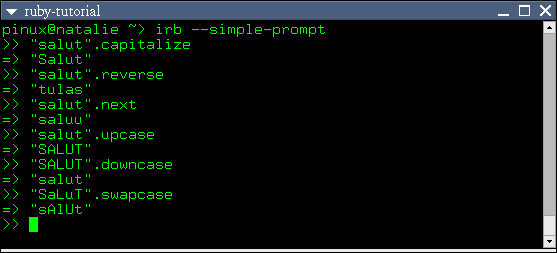
\includegraphics[width=1\linewidth,center]{img/methode-chaine.png}\\
\\
Voici la liste des classes Ruby de base:\\
\\
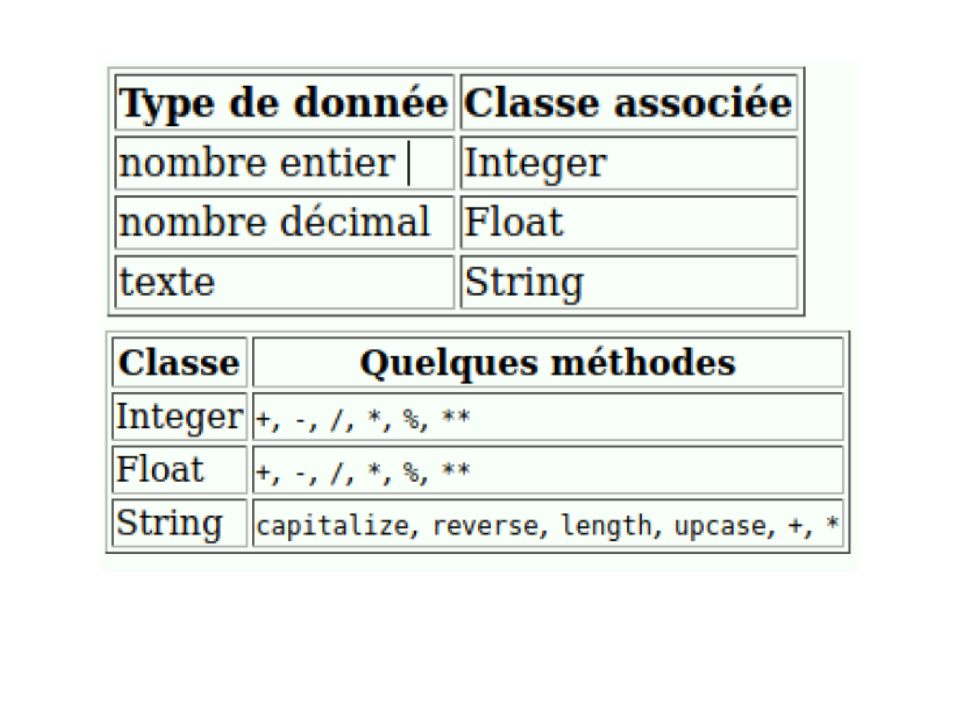
\includegraphics[width=1\linewidth,center]{img/classe-methode-debase.png}\\
\\
Voici la liste des quelques methodes effectuant des conversion sur les chaines:\\
\begin{tabular}{|c|c|c|}
\hline
Methode & Description \\ \hline
to_i & string converti en entier \\
to_i & flottant converti en entier \\ \hline
to_f & string converti en flottant \\ 
to_f & entier converti en flottant \\ \hline
to_s & flottant converti en string \\ 
to_s & entier converti en string \\ \hline
\end{tabular}
\\

%%%%%%%%%%%%%%%%%%%%%%%%%%%%%%%%%%%%%%%%%%%%%%%%%%%%%%%%%%%%%%%%%%%%%%%%%%%%
\section{Condition if-else-elsif}

Peux s'employer avec les operateur de comperaison : \textbf{and},\textbf{or},\textbf{not}.\\
\\
\begin{verbatim}
age=17
if age < 17  
  print 'vous etes mineur'
else if age > 18 and age <= 100
  print 'vous etes majeur'
else
  print 'vous etes un senior'
end
\end{verbatim}
\\
Lors de plusieur comparaison dans la condition l'ajout ou non de parenthése peux changer le resultat de la condition, on modifie l'ordre de priorité des opérations. Ex:\\
(1 == 1 || 2 ==3) && 3==4 vaut false\\
1 == 1 || (2 ==3  && 3==4) vaux true\\
\\
La structure \textbf{unless}

%%%%%%%%%%%%%%%%%%%%%%%%%%%%%%%%%%%%%%%%%%%%%%%%%%%%%%%%%%%%%%%%%%%%%%%%%%%%

\section{Boucle}

\subsection{while}
\begin{verbatim}
compteur = 0

while (compteur <= 4)
  print compteur
  compteur += 1
end
# => 0 1 2 3 4
\end{verbatim}

%%%%%%%%%%%%%%%%%%%%%%%%%%%%%%%%%%%
\subsection{loop}
\begin{verbatim}
n = 0

loop
 {
  print n
  n += 2
  break if (n > 6)
 }
# => 0 2 4 6
\end{verbatim}

%%%%%%%%%%%%%%%%%%%%%%%%%%%%%%%%%%%

\subsection{until}

La boucle until est à la boucle while ce que unless est à if. Cette boucle s'exécute jusqu'à ce qu'une condition soit vraie. Elle est donc totalement équivalente à while!(condition). \\
\\
\begin{verbatim}
n = 0

until n>5
  print n
  n += 2
end
# => 0 2 4
\end{verbatim}

%%%%%%%%%%%%%%%%%%%%%%%%%%%%%%%%%%%

\subsection{for}

La boucle for exécute des instructions données pour chaque élément d'un ensemble.\\
\\
\begin{verbatim}
for n in (0..7)
do (do est facultatif)
  print n," "
end
# => 0 1 2 3 4 5 6 7
\end{verbatim}
\\
cela marche aussi avec de chaine de caractere:\\
\\
\begin{verbatim}
for s in "a".."g"
  print n," "
end
# => a b c d e f g
\end{verbatim}

%%%%%%%%%%%%%%%%%%%%%%%%%%%%%%%%%%%

\subsection{Autre maniere de faire des boucles}

\texbf{upto}:\\
Pour la classe Enumerable et String.\\
\begin{verbatim}
5.upto(10) {|i| print i, " " }   
#=> 5 6 7 8 9 10

#ou

5.upto(10) do |i|
  print i," "
end
#=> 5 6 7 8 9 10
\end{verbatim}
\\
Version avec chaine de caratere:\\
\begin{verbatim}
"a8".upto("b6") {|s| print s, ' ' }
#=> a8 a9 b0 b1 b2 b3 b4 b5 b6
\end{verbatim}
\\
\\
\texbf{time}:\\
Utilise la classe Time.\\
\begin{verbatim}
10.times { puts "hello" }
=>Affichera 10 fois hello
\end{verbatim}
\\
\\
\texbf{each}:\\
Fonctionne avec des collection, classe Array.\\
\begin{verbatim}
numbers = [1, 3, 5, 7]
numbers.each #Affichage tableau (marche mais pas recommander)
#ou
numbers.each { |n| puts n } #affichage a chaque ligne
#=> 1 3 5 7
\end{verbatim}


%%%%%%%%%%%%%%%%%%%%%%%%%%%%%%%%%%%%%%%%%%%%%%%%%%%%%%%%%%%%%%%%%%%%%%%%%%%%

\section{Definition de Variable/Methode/Class}

\textbf{Une variable} se declare simplement par son nom, elle ne seras pas typé on peux donc faire:\\
\\
\begin{verbatim}
$irb
$var1=7
$=>7
$var2="salut"
\end{verbatim}
\\
\textbf{Les constante} se comportent comme des variables sauf qu'a leur déclaration leur nom doit commencer par une majuscule "Constante".\\
Cela ne permettra pas a la variable de ne pas etre modifie mais indiquera a ruby de nous avertire (avec un message d'erreur) si notre variable est modifié.\\ 
Il existe des constante prédéfinie dans ruby tel que : Pi, Masse_electron, Distance_terre_soleil, etc.\\
\\

%%%%%%%%%%%%%%%%%%%%%%%%%%%%%%%%%%%

\subsection{Méthode}

Voici quelque méthode connue prédéfini de Ruby:\\
\\
-\textbf{puts} : Méthode qui affiche une chaine de caractere.\\
\emph{Utilisation}: puts(String)\\
\underline{Ex}:\\
nom="Mateo"\\
puts "Bonjour!!!" + nom + "Le boss"\\
\$=>Bonjour!!! Mateo Le boss\\
\\
Attention: Si on peux afficher un entier avec puts il faudra le convertir en string avant de pouvoir l'afficher sinon cela provoquera une erreur.Ex:\\
\begin{verbatim}
y=30-10
puts "Le resultat de y est " + y          %ERREUR
puts "Le resultat de y est " + y.to_s     %OK
\end{verbatim}
\\
%%%%%%%%%%%%%%%%%%%%%%%%%%%%%%%%%%%

\subsection{Classe}

On peux inclure une classe a partir d'un autre fichier rb grace au mot cle "load".\\
Exemple : load 'nom\_fichier' \# sans l'extension du fichier .rb\\
\\
Une classe se definie avec le mot cle "class nom\_class" et se fini par "end".\\
\\
\textbf{SuperClasse}\\
L'objet de la methode #class() method returns the claretourne la classe qui a instancier l'objet.\\
Toutes les classe en Ruby sont une instance de la Class class.\\
\begin{verbatim}  
Object.class # => Class
class A; end
A.class # => Class
\end{verbatim}
\\
L'instanciation de classe varient pour tout objet en Ruby ce ne sont pas des class objects.\\
\begin{verbatim}
class A; end
A.new.class # => A
{}.class # => Hash
4.class # => Fixnum
\end{verbatim}
\\
Voici une représentation de la hiearchie des classes en Ruby:\\
\\
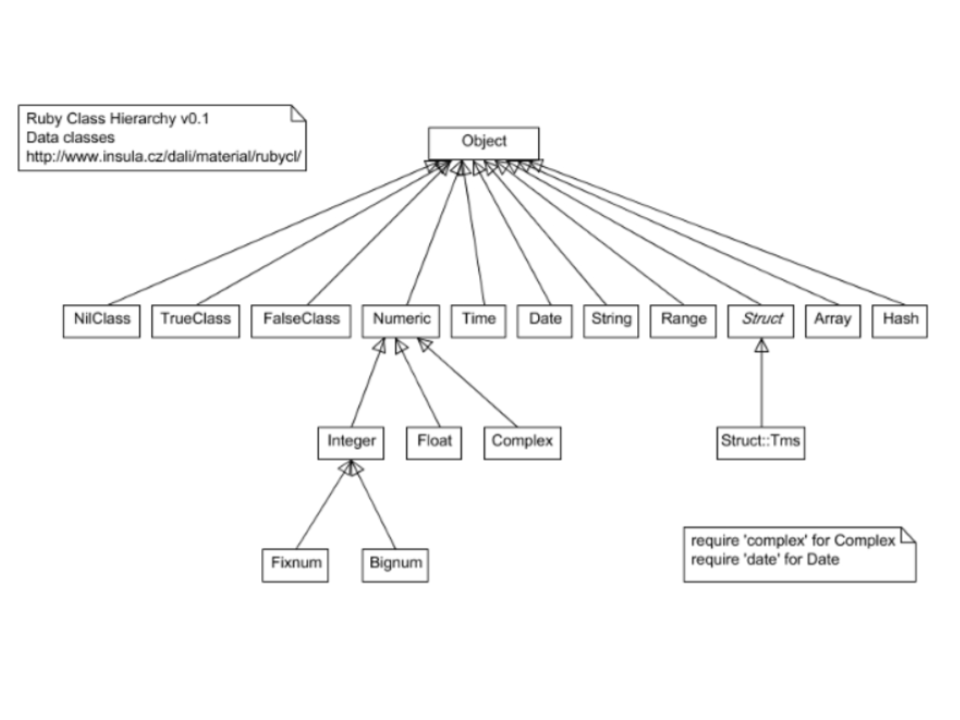
\includegraphics[width=1\linewidth,center]{img/ruby-class-hierachie-data.png}\\
\\
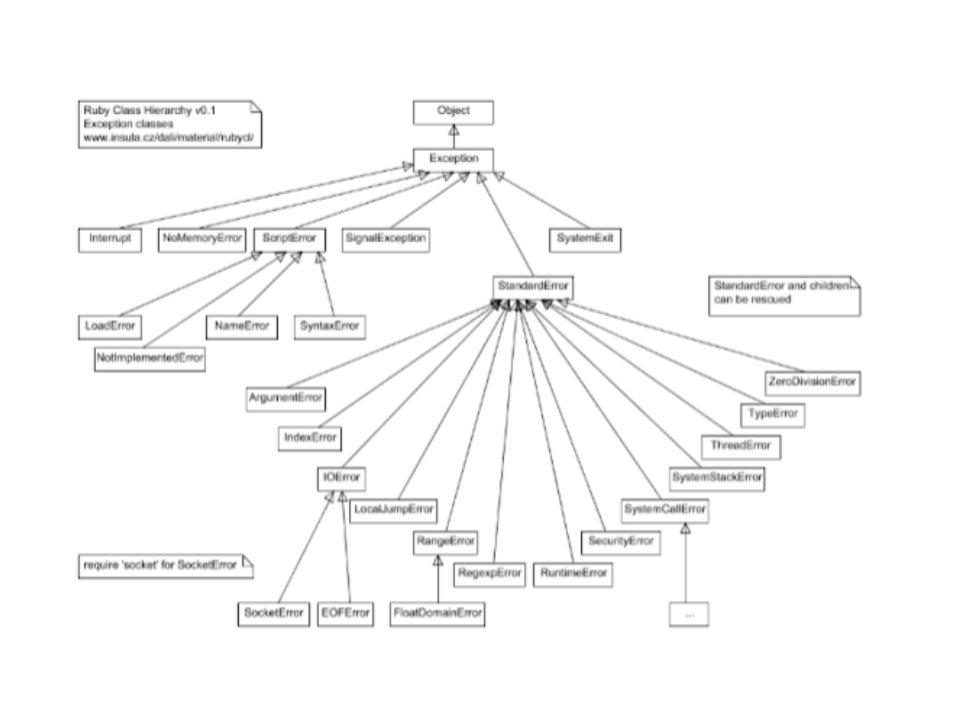
\includegraphics[width=1\linewidth,center]{img/ruby-class-hierachie-exeption.png}\\
\\
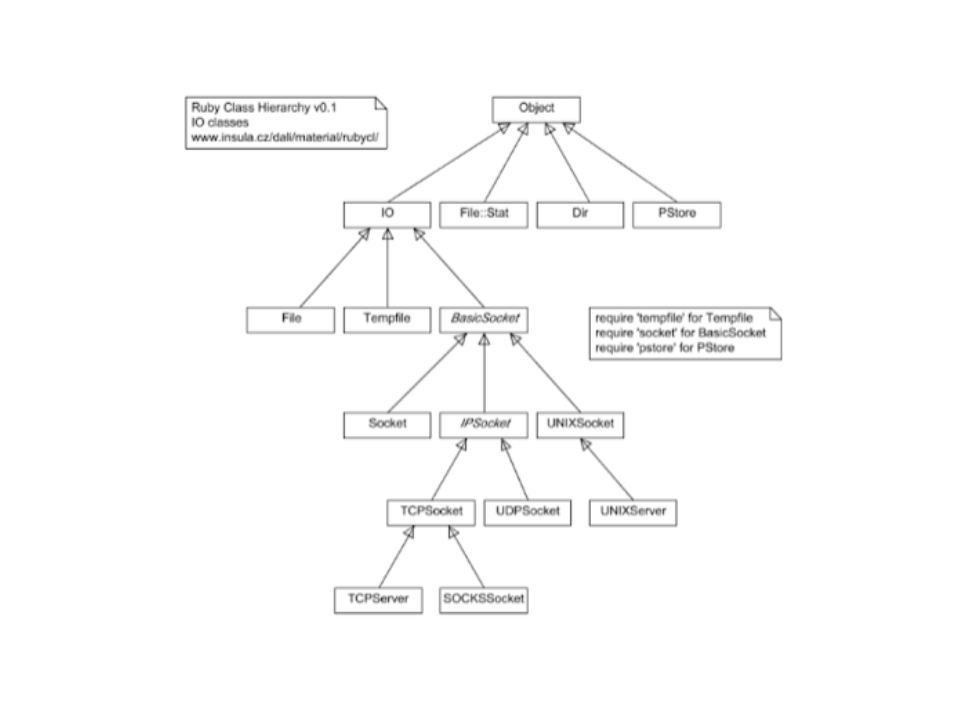
\includegraphics[width=1\linewidth,center]{img/ruby-class-hierachie-io.png}\\
\\
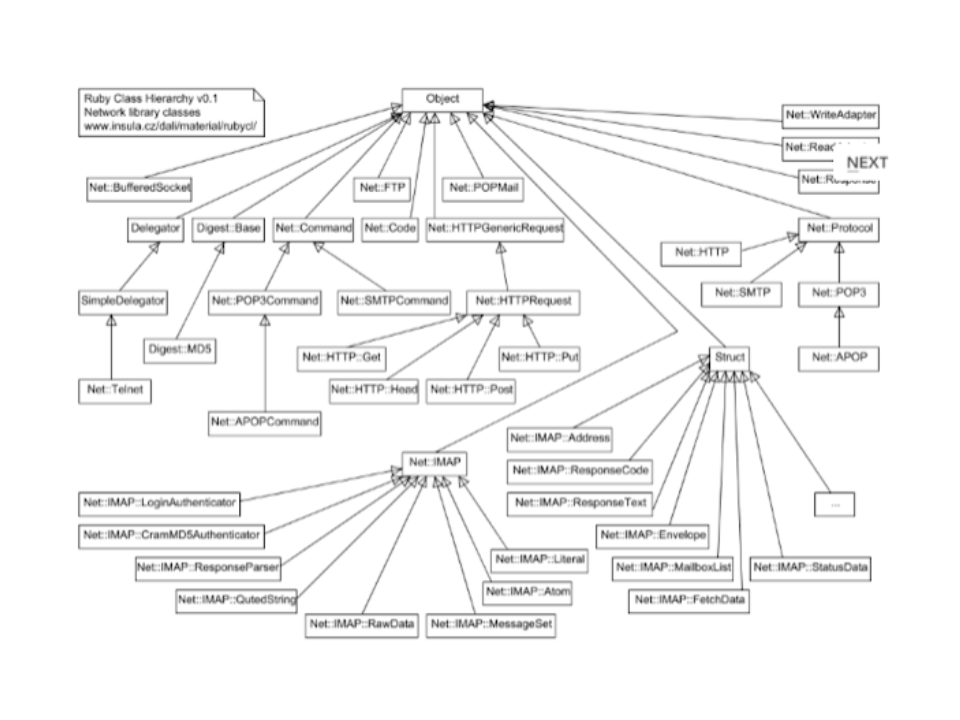
\includegraphics[width=1\linewidth,center]{img/ruby-class-hierachie-networkLib.png}\\
\\



%%%%%%%%%%%%%%%%%%%%%%%%%%%%%%%%%%%%%%%%%%%%%%%%%%%%%%%%%%%%%%%%%%%%%%%%%%%%

\section{Bloc}

Utilisation d'accolade ouvrante,fermante {bloc}. Un bloc permet d'executer une suite d'instruction.\\
Un bloc bloc peut etre utiliser dans une strucrture de répétition.\\
Exemple:\\
0.upto(9) {print "salut"}  => 0.upto(9) do print for "salut". Le bloc agit comme une sorte de parametre a la fonction upto.\\
\\
Un bloc peut avoir des parametre, déclarer entre "|param|". 0.upto(9) {|param| print param}. \\
Le mot clé "yield" permet d'appeler un bloc de code. Exemple:\\
\begin{verbatim}
def deux_fois
  yield
  yield
end

deux_fois {puts "Vive ruby!!"}

Resultat:
Vive ruby!!
Vive ruby!!
\end{verbatim}

On peux stocker un bloc dans une variable c'est ce qu'on appele un "objet procédure".\\



%%%%%%%%%%%%%%%%%%%%%%%%%%%%%%%%%%%%%%%%%%%%%%%%%%%%%%%%%%%%%%%%%%%%%%%%%%%%%%%%%

\section{Collection}

Les collection fournissent des services pour manipuler des données qu'elle contient.\\
La classe Array représente une collection d'items.\\


%%%%%%%%%%%%%%%%%%%%%%%%%%%%%%%%%%%%%%%%%%%%%%%%%%%%%%%%%%%%%%%%%%%%%%%%%%%%%%%%%

\section{Tableaux}

Un tableau peut etre manipuler comme une liste.\\
Methode sur les tableau: .class, .upcase, .reverse, .sort, .length\\
\\
Array.new([Taille=0][,remplissage])
Intersection \& \\
Union \| \\
Concaténation \* \\
\\
Acces a un element: [1,2,3].at(1) => 2\\
\\
Manipulation d'un tableau: \\
-a.first a.last: Retourne le premier/dernier element \\
-a.push(val) -> ajout en fin de tableau\\
-a.pop -> retire en fin de tableau\\
-a.shift -> retire au debut du tableau \\
-a.unshift -> ajout au debut valeur du tableau \\
-a.clear: Supprime tout les elements du tableau\\
-a.uniq: Supprime les doublons a l'affichage\\
-a.uniq!: Supprime les doublons dans le tableau (! methode destructive, a definir le ! fait partie du nom de la methode)\\
-a.delete (e): Supprime tout les element du tableau \\
-a.delete (e) {|e|...}: Si aucun element supprimé renvoie l'évaluation du bloc.\\
-a.delete_at(n), a.delete_if {|x| ... } \\



%%%%%%%%%%%%%%%%%%%%%%%%%%%% JAVA %%%%%%%%%%%%%%%%%%%%%%%%%%%%%%%

\chapter{JAVA}

Tout comme Ruby , JAVA est un langage de programmation orienté objet. La plupart des langages de programmation moderne dispose d'un generateur de documentation JAVA fournie ca propre documentation du code appelé javadoc .

JVM (Java Virtual Machine), JDK (Java Development Kit) et JRE (Java Runtime Environment) sont trois composants indispensables de la plate-forme Java. Ils fonctionnent ensemble dans les applications Java.

En bref, la machine virtuelle Java ou JVM est le composant de la plate-forme Java qui exécute les programmes ; l’environnement de développement Java ou JRE crée la machine virtuelle Java ou JVM et s'assure que les dépendances sont disponibles pour les programmes Java ; le kit de développement Java ou JDK permet de créer des programmes Java qui peuvent être exécutés par la JVM et le JRE.

Les développeurs utilisent le JDK pour écrire leurs applications et la JVM pour les déboguer et les optimiser, améliorer les performances en particulier. Le JRE tourne essentiellement en arrière-plan, mais il est possible de l'utiliser pour surveiller les applications et configurer la mémoire.

\section{Synthaxe}

Les types primitifs = booleens, caracteres, entiers, reels.
Une variable de type primitif est manipulee par valeur
Une variable de type non-primitif est manipulee par reference.

La synthaxe de java se rapproche plus du C que de Ruby , respecte des delimiteurs , type de variable.
\begin{verbatim}
public class MyVariable {

	public static void main(String[] args) {
	   int var = 500;
	   ...
	}
}
\end{verbatim}

\\
Constant : mot clef final (final int entier = 9;).
Operation : Comme en ruby \verb!+=,-=,/=,*=! .
\\
En JAVA le compilateur intervient en amont pour interpréter le code et le transformer en byteCode (ou code binaire). Puis l'interpréteur traduit le byteCode en instructions pour exécuter le programme.

Le langage dans lequel le code Java doit être transformé est appelé Bytecode. Pour transformer le code Java en Bytecode, il est nécessaire d'utiliser le compilateur javac.
\\

En Java, il y a une correspondance directe entre :

les packages et les dossiers.
les classes et les fichiers.

- Pour compiler un programme java en ligne de commande il faut faire 'javac nom.java' , ensuite on peut l'executer avec la commande 'java'.

Lorsque l'on veux creer un objet , la rocedure est comme en ruby grace au mot clef 'new' , exeple : 
MyVariable variable = new MyVariable();
\\
Porté :

-public : visible pour tous et par conséquent le moins restrictif ;
-protected (protégé) : visible pour le package et l'ensemble de ses sous-classes ;
-package-protected (protégé par paquet) : généralement visible uniquement par le package dans lequel il se trouve (paramètres par défaut) ;
-private (privé) : accessible uniquement dans le contexte dans lequel les variables sont définies (à l'intérieur de la classe dans laquelle il est situé).

static: Une variable declaree static est une variable de classe: commune a toutes les instances de la classe. a contrario on a des variable/methode non-static qui elle peuvent utilisé "this" car ils s'agit d'une reference a une instance.
Le mot-clé static devant une variable (ou méthode) indique que celle-ci n'appartient pas à une instance particulière de la classe. Les variables ou méthodes statiques appartiennent à la classe elle-même. On peut ainsi les utiliser sans avoir une instance créée. De nombreuses classes ont des membres ou méthodes statiques. Par exemple la classe java.lang.Math :


\sectio{Classe abstraite}

Une classe abstraite ne peux pas etre instancier , elle peux disposer de methodes abstraite qu'on ne definie pas a l'implementation on laisse le corp de la methode vide (comme une sorte de header en C) , la methode seras defini dans les classe qui etendron de cette classe bastraite , par exemple : 
 une classe bastraite formeGeometrique qui dispose de la methode perimetre() mais comment appliquer les bonnes formules ? pour cela la classe Cercle et Carre vont etendre l(extend) la classe abstraite Forme pour redefinir leur propre methode perimetre.

\section{Interface}

Une interface est une classe abstraite définie par le mot clé interface. (abstract est implicite)
– Toutes les méthodes d’une interface sont abstraites , on ne peux donc pas l'instancier (pas de new).
– Les seules attributs autorisés sont des constantes de classe. (static et final implicites) , Tous les champs sont public static final.


Une classe Fille ne peut hériter que d’une classe mere mais une classe peut implémenter plusieurs interfaces (héritage de comportement).
Une interface permet d'eviter l'héritage multiple qui n'est pas autorisé en JAVA.

L'implementation d'une interface a une classe se fait avec le mot clé "implements" , exemple : 
Class Chauffeur extends Employe implements Representable {....}

Une interface ne peut contenir que des attributs constants (static final) et des méthodes publiques non implémentées.

Une classe peut implémenter (implements) une ou plusieurs interfaces tout en héritant (extends) d'une seule classe :
public maClasse extends MaClasseMere implements Interface1, Interface2{...}

Une interface peut hériter (extends) d'une autre interface
– les interfaces forment une hiérarchie séparée de celle des classes : hiérarchie de comportements

\section{methode}

Methode de comparaison :

On peux comparer avec le signe "==" avec 2 variable de type primitif car ce sont 2 references qui point au meme endroit mais si on veux tester l'egalité en terme de valeur/contenue il faut utiliser la method equals() .

int[] S={1,2,3};
int[] T={1,2,3};
int[] U=T;
System.out.println((S==T) + "," + (T==U));
Affiche: false,true

Pour tester l’´egalite des contenus pointes, utiliser la methode equals.

int [] T = {1, 2, 3} ;
boolean b = T.equals(new int [] {1, 2, 3});
System.out.println(b);
Affiche: true


\end{document}